\section{Application \& Use Cases}

\subsection{\ours Application}

To demonstrate the full functionality of our memory system, we developed a cross-platform application using \texttt{React-Electron} for the frontend and \texttt{Uvicorn} as the backend server. Moreover, we release the obtained file for direct installation. Within the application, users can activate screen monitoring by selecting the \texttt{ScreenShots} tab. This enables the agent to observe the user’s screen activity and dynamically update its memory, gradually building a contextual understanding of the user over time. With the obtained memory, the agent can answer questions related to the memories.

\paragraph{Memory Updates}
The application captures a screenshot every 1.5 seconds. To reduce redundancy, images that are visually similar to previously captured ones are discarded. Once 20 unique screenshots are collected, the memory update process is triggered—typically around every 60 seconds. During this process, relevant information is extracted and incorporated into the system's memory components. To reduce latency in processing user screenshots, we adopt a streaming upload strategy. Instead of batching and sending 20 images at once, we upload each screenshot immediately upon receiving it from the front-end. By leveraging the Gemini API—which supports loading images via Google Cloud URLs—we can efficiently transmit visual data without waiting for the full batch to accumulate. This approach significantly reduces end-to-end latency from approximately 50 seconds (as observed when using GPT-4 with direct image upload) to under 5 seconds using Gemini.


\paragraph{Chat Interface}
The chat interface allows users to interact with the agent, which has full access to its accumulated memories. As illustrated in Figure~\ref{fig:chat_window}, users can query the assistant about past activities, and the agent can respond based on its memory content, enabling more informed and personalized interactions.


\begin{figure}[t]
    \centering
    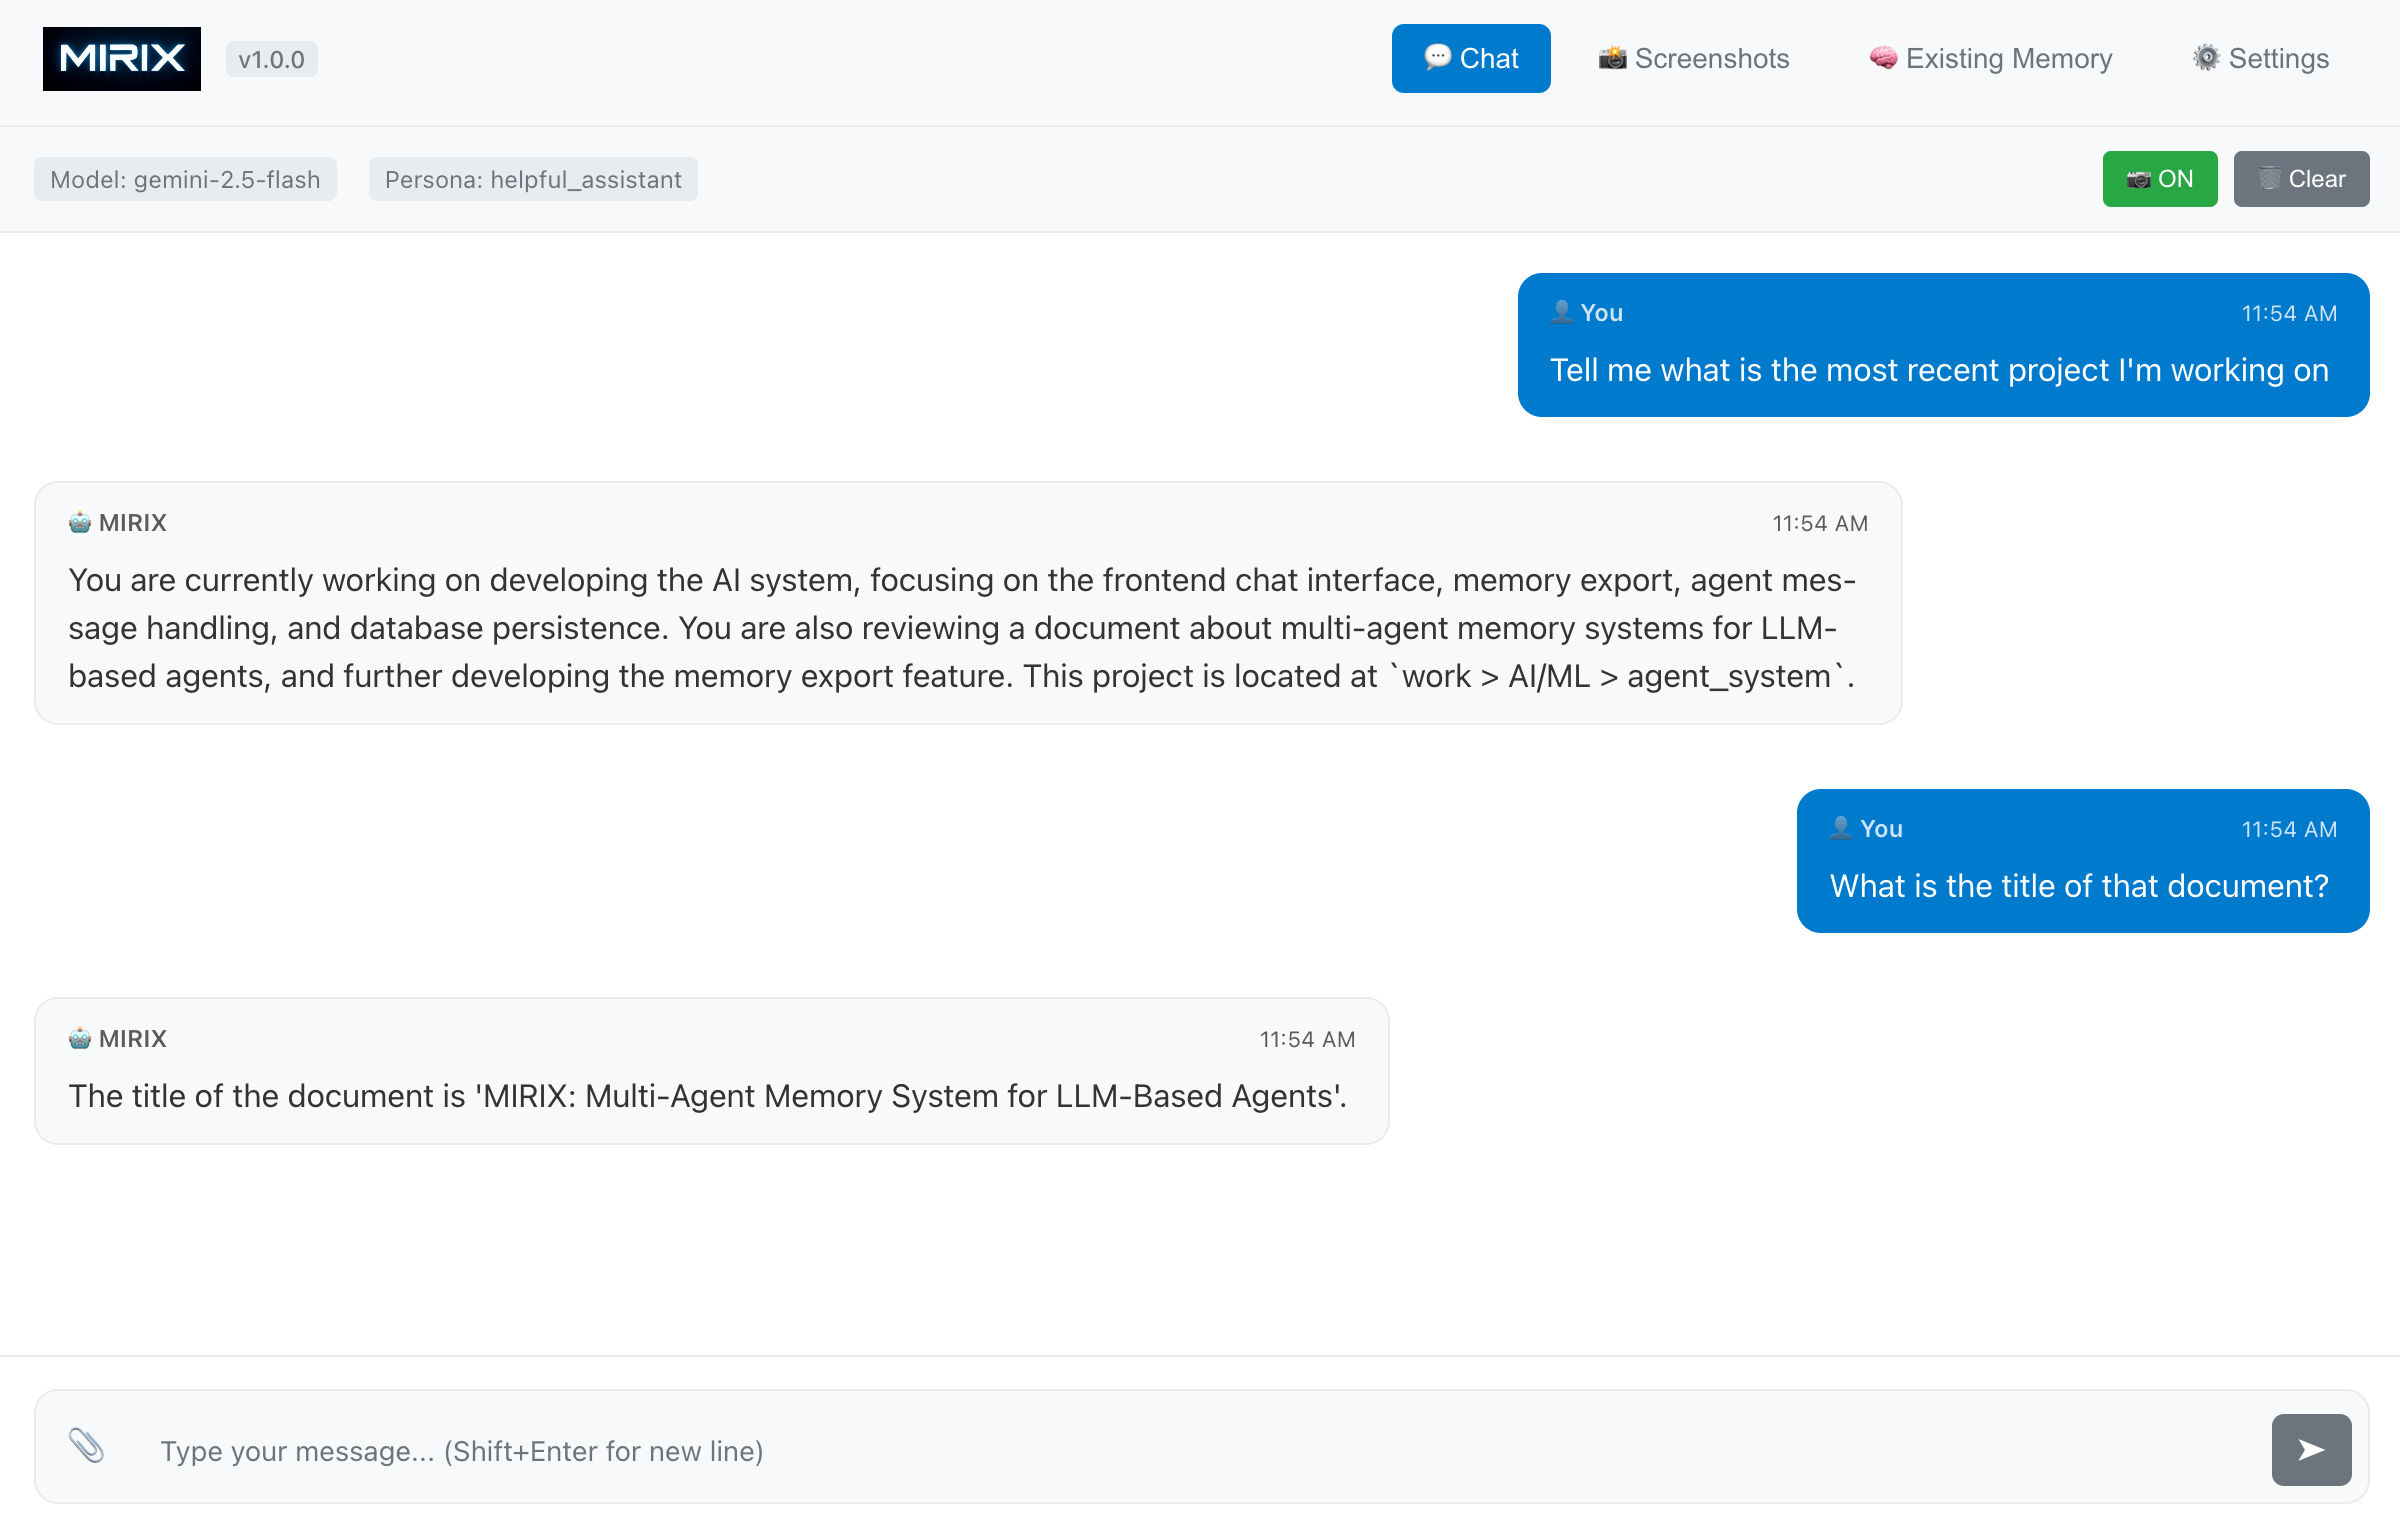
\includegraphics[width=0.95\linewidth]{figures/chat.png}
    \caption{Chat Window}
    \label{fig:chat_window}
\end{figure}


\paragraph{Memory Visualization}
After observing the screen for a sufficient period, the agent organizes its knowledge into structured memory components. An example of Semantic Memory (organized into a tree structure) is shown in Figure~\ref{fig:semantic_tree}. We also provide a list view of the memories. An example of Procedural Memory is shown in Figure \ref{fig:procedural_list}. 


\subsection{Memory System for Wearable Devices}
The wearable device market has seen rapid growth in recent years, driven by the increasing demand for intelligent, always-available personal assistants. Products like AI-powered glasses (e.g., Meta Ray-Ban, XREAL Air) and AI pins (e.g., Humane, Rabbit R1) aim to integrate seamless interaction into daily life through voice commands, visual capture, and real-time feedback. However, these devices often lack a long-term memory component that allows them to evolve with the user—retaining useful information over time, adapting to personal routines, and referencing past interactions in context-aware ways.

Our memory system is well-suited for integration into such wearable devices. By continuously collecting and processing data streams such as audio, visual scenes, and user queries, our system enables real-time memory formation. For instance, AI glasses equipped with our memory systems can automatically summarize meetings, remember frequently visited places, recognize recurring visual patterns, and recall previous conversations or tasks. With \ours, it can also evolve with the user and build a memory that is specifically made for the user. 
Moreover, the system’s modular memory architecture—including procedural, episodic, semantic, and resource memory—aligns naturally with the needs of lightweight, on-the-go devices. Procedural memory enables the assistant to learn user habits (e.g., daily routes, meeting structures), while semantic memory stores general knowledge about the user's preferences, environment, and routines. Episodic memory captures time-stamped, situational experiences, and can be queried for recalling specific events (e.g., “What did I see at the conference last week?”). Semantic Memory, on the other hand, can help organize the clients someone has seen over the past week and list them in a tree structure with details of their discussions.

Given the constraints of wearable hardware (limited compute and storage), our design also supports hybrid on-device/cloud memory management. Critical information in Knowledge Vault can be stored locally while large-scale memories such as Resource Memory can be offloaded and retrieved from the cloud on demand. 

In summary, our memory system serves as a cognitive backbone for wearable AI agents—enabling personalization, continuity, and intelligence at the edge. As the wearable market matures, embedding persistent, structured memory will be a key differentiator for next-generation AI assistants.

\subsection{Agent Memory Marketplace}
We envision a future where personal memory—collected and structured through AI agents—becomes a new digital asset class. In the AI era, memory is no longer just a passive log of past events, but an active, evolving knowledge base that can be shared, personalized, and monetized. The Agent Memory Marketplace is our proposal for a decentralized ecosystem where memory is exchanged, reused, and built collaboratively through AI agents. 


\begin{figure}
    \centering
    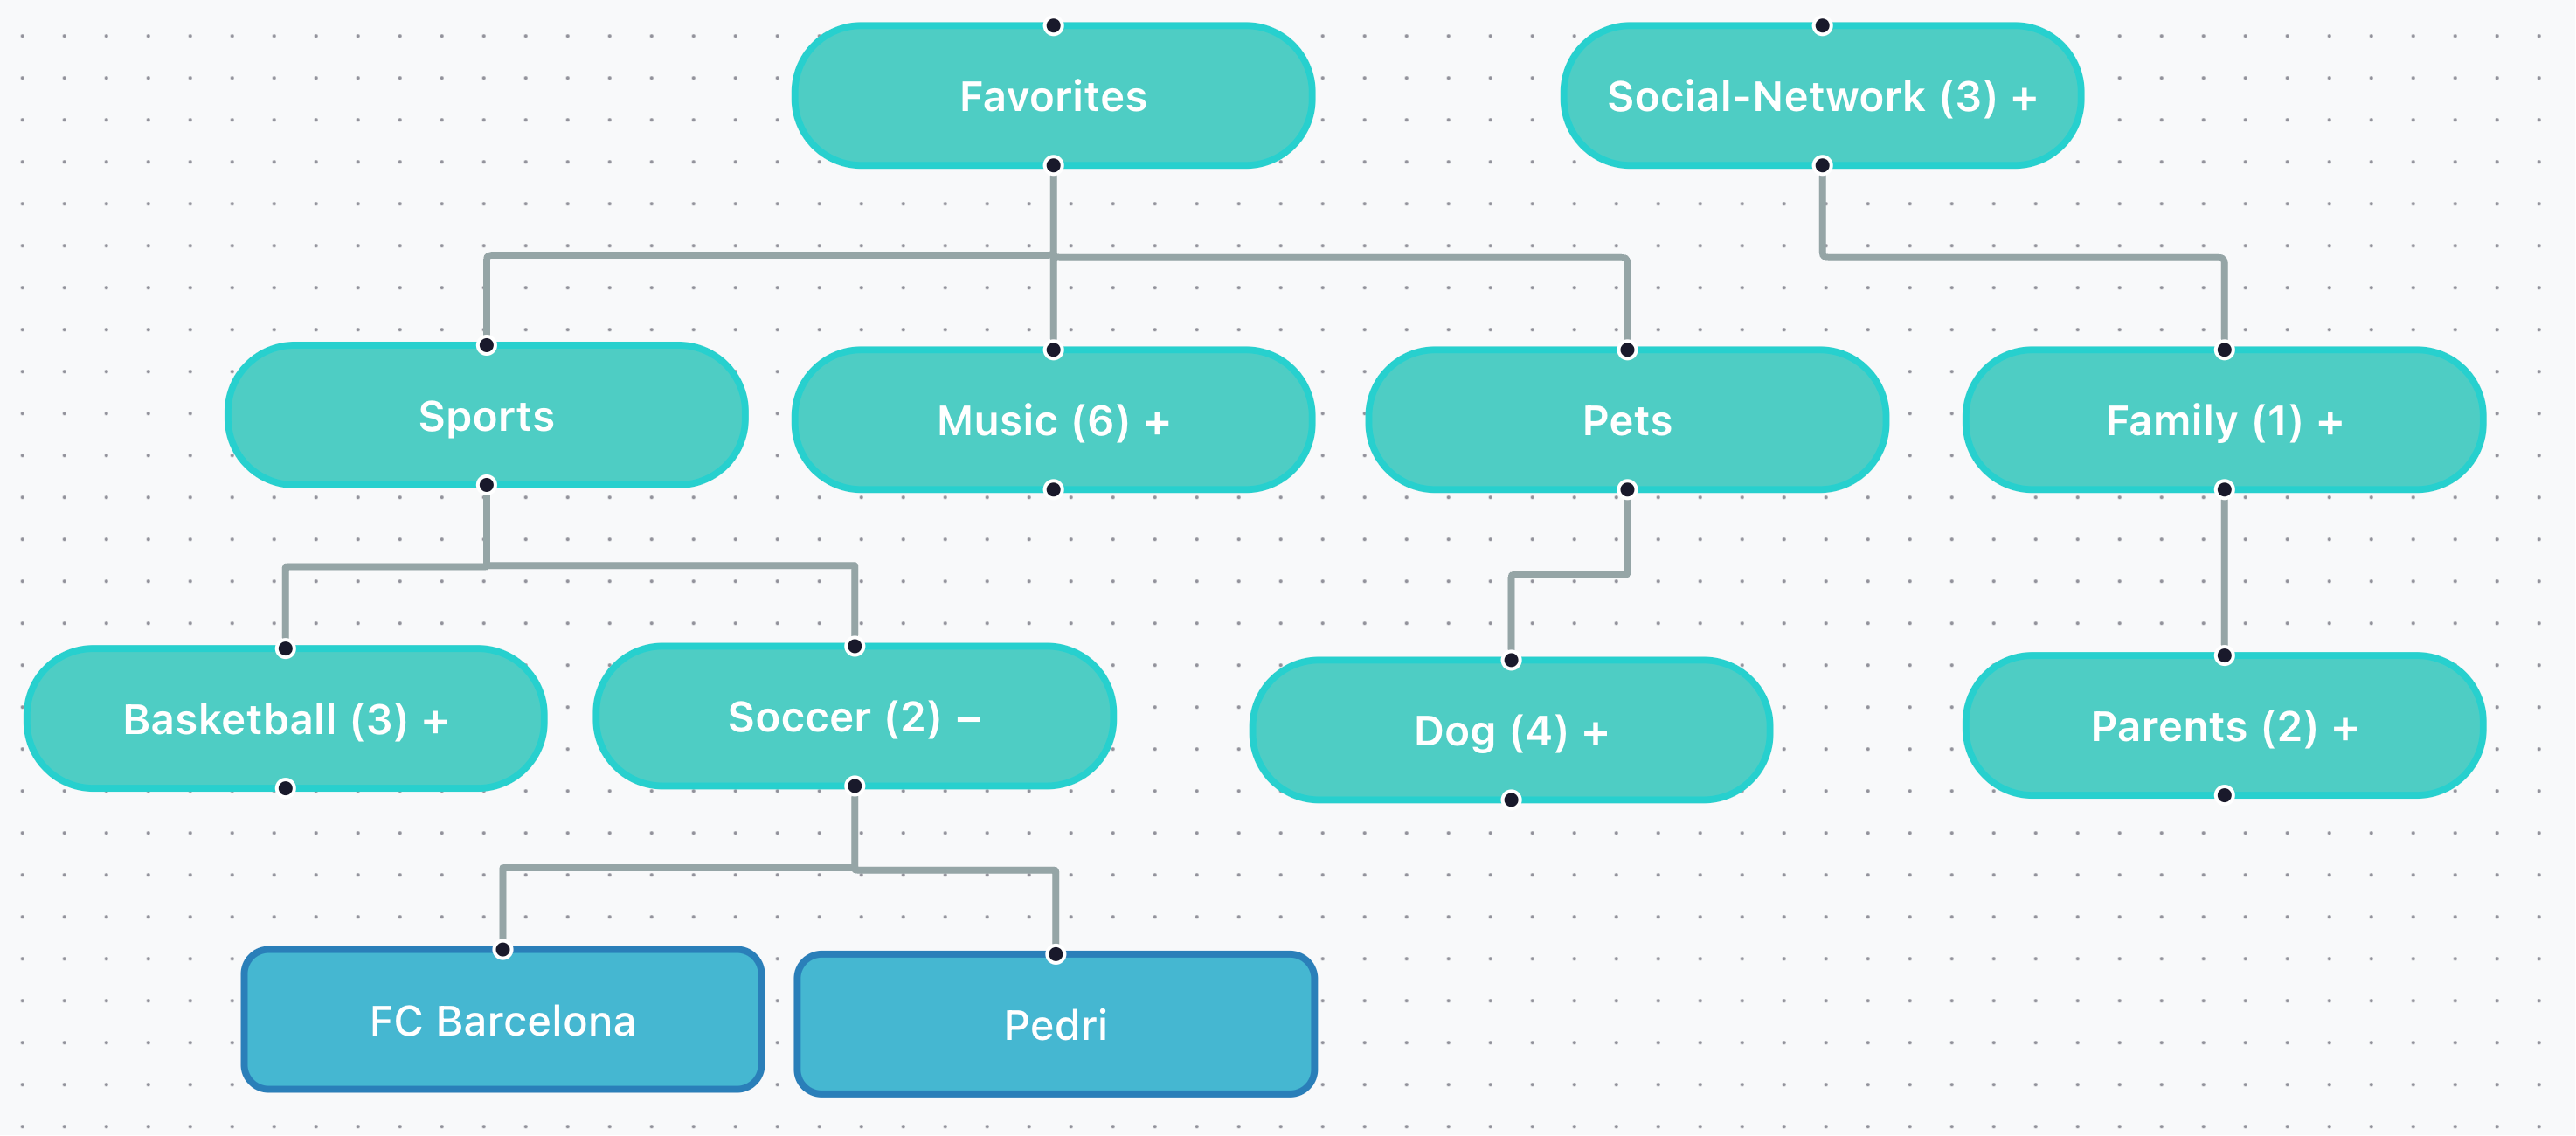
\includegraphics[width=1.0\linewidth]{figures/semantic_tree.png}
    \caption{Tree Structure of an Example Semantic Memory. In this example, the user's Semantic Memory, which stores new concepts and their relationships, is organized hierarchically into multiple categories, such as \emph{Social Network} and \emph{Favorites}. Within \emph{Favorites}, the memory is further divided into more specific classes, including \emph{Sports}, \emph{Pets} and \emph{Music}.}
    \label{fig:semantic_tree}
\end{figure}

\begin{figure}
    \centering
    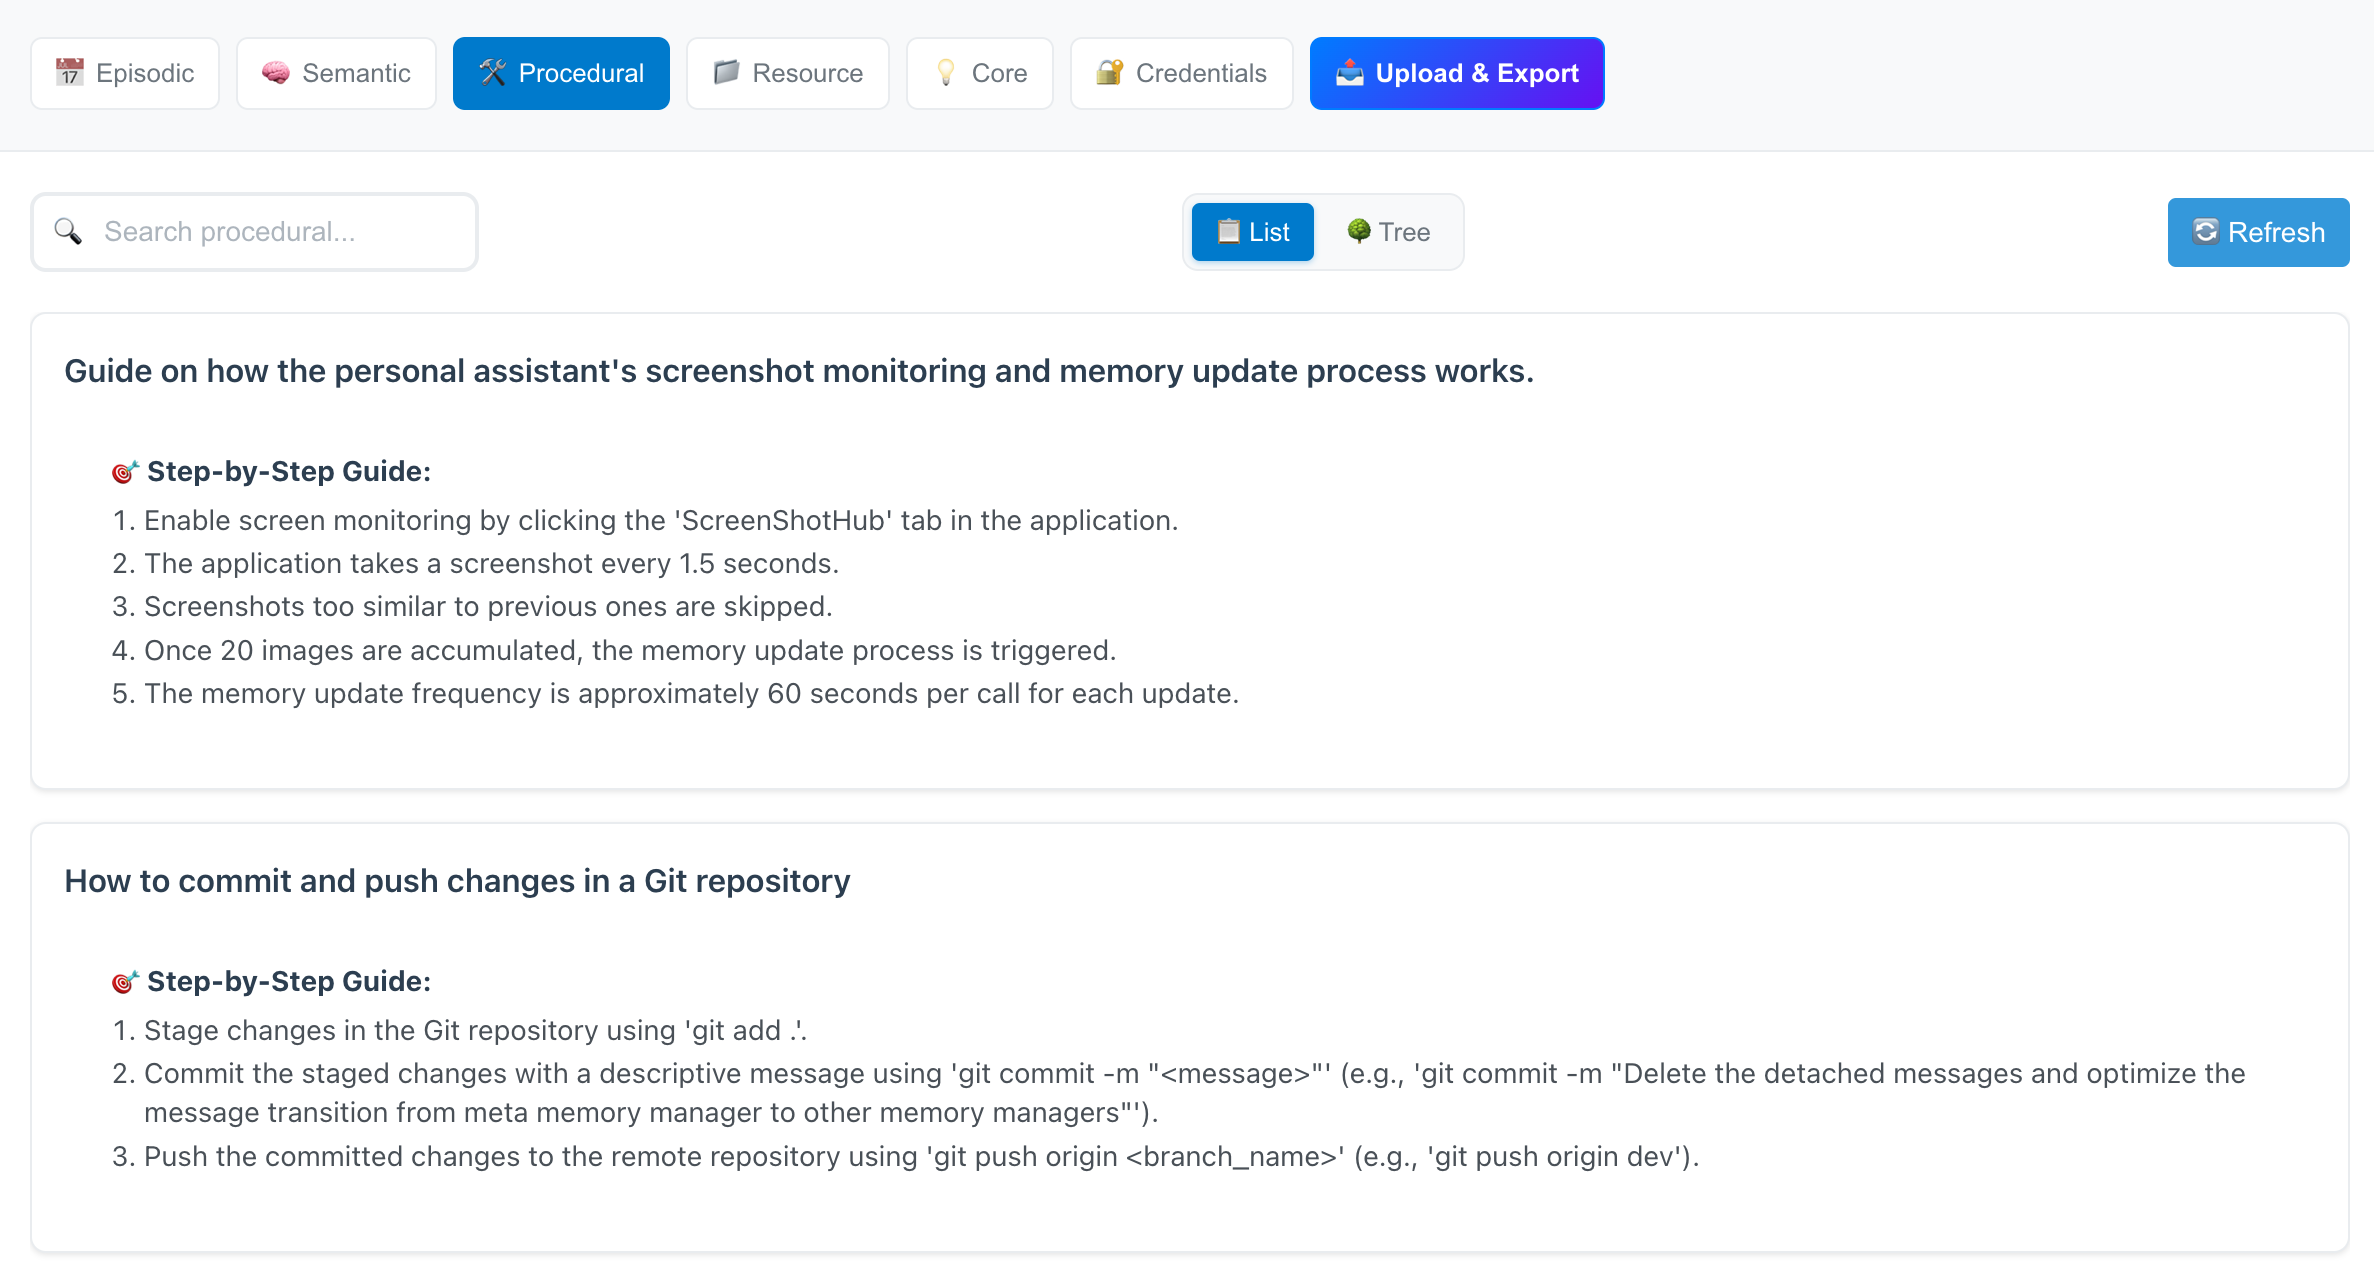
\includegraphics[width=1.0\linewidth]{figures/procedural_list.png}
    \caption{List View of an Example Procedural Memory.}
    \label{fig:procedural_list}
\end{figure}



We begin with a core belief: \textbf{human memory will become the most valuable and irreplaceable asset in the age of AI}. Unlike static data, memory encompasses lived experiences, subjective context, preferences, and interactions—making it deeply personal, yet highly reusable by intelligent systems. the marketplace is structured into three key layers:

\begin{enumerate}[leftmargin=*]
    \item \textbf{AI Agents Infrastructure}. Our technology provides infrastructure for lifetime intelligent, interactive agents. Examples include (1) Personal AI Assistants \& Companions: Tailored agents that continuously learn and evolve with the user. (2) AI Wearables: AI agents embedded in decentralized physical infrastructure (e.g., smart glasses, AI pins) that extend memory capture to the real world. (3) Multi-Agent Systems: Collaborative agents with shared memory access, enabling coordination and collective intelligence.
    \item \textbf{Privacy-Preserving Memory Infrastructure} To support trust and adoption, we aim to build in a robust privacy layer: (1) Encryption Layer: All memories are stored using end-to-end encryption. (2) Privacy Control: Fine-grained permissions allow users to choose which parts of their memory to share, trade, or restrict. (3) Decentralized Storage: Memories are stored in a distributed, censorship-resistant infrastructure.
    \item \textbf{Memory Marketplace and Social Function}: A peer-to-peer ecosystem for sharing, aggregating, and trading memories encoded in AI agents. Use cases include: (1) Memory Social/Trading: Tokenized exchange of memories (e.g., productivity hacks, niche workflows, or life advice). (2) Expert Communities: Collective memory-building for domain-specific expertise such as finance, education, or pet care. (3) Fan Economy and Dating Applications: Users can subscribe to AI personas based on influencer or celebrity memories, allowing fans to interact with memory-rich digital replicas of their favorite personalities. This technology also enables the creation of AI clones for accelerated dating and matching processes, where users can engage with AI agents in interactions before meeting in person.
\end{enumerate}

In summary, we envision a future where personal memory transcends its traditional role to become an active, valuable digital asset. By combining lifelong AI agents, privacy-preserving infrastructure, and a decentralized marketplace, we aim to create an ecosystem where memories can be securely captured, meaningfully shared, and collectively advanced. This approach not only empowers individuals to benefit from their own experiences but also unlocks new possibilities for collaboration, personalization, and economic value in the AI era.







